\documentclass[10pt,a4paper]{article}
\usepackage[utf8]{inputenc}
\usepackage{amsmath}
\usepackage[margin=1.15in]{geometry}
\usepackage[pdftex]{graphicx}
\usepackage{amsfonts}
\usepackage{amssymb}
\usepackage{hyperref}
\hypersetup{
    colorlinks=true,
    citecolor=black,      
    urlcolor=cyan,
}
\usepackage[T1]{fontenc}
\renewcommand*{\figurename}{Rys.} 
\renewcommand*{\tablename}{Tab.} 
\author{Rafał Kornel}
\title{\textbf{Badanie układu RC - filtra dolnoprzepustowego / układu całkującego.}}
\date{}
\begin{document}
\maketitle

\section*{Abstrakt}
Celem niniejszego doświadczenia było zbadanie własności prostego układu całkującego - 
filtra dolnoprzepustowego. Zbadana została hipoteza głosząca, że układ szeregowy 
złożony z opornika i kondensatora będzie przepuszczał prąd o małej częstości 
drgań, oraz że tenże układ dla prądów o częstości znacznie większych od pewnej 
częstości granicznej na wyjściu będzie zwracał prąd, którego kształt jest zcałkowanym
sygnałem wejściowym. Obie hipotezy zostały potwierdzone, ponadto została dopasowana
częstość graniczna wynosząca 
$$ f_k = 1712.6 \pm 5.6 \ \text{Hz}. $$ Dla zmierzonych wartości $R$ oraz $C$ policzono wartosć krytyczną częstotliwości, wynosi ona:
$$ f_{zm} = 1660 \pm 11 \ \text{Hz}.$$ Udało się również na podstawie punktów pomiarowych wyznaczyć
współczynnik $RC$, pojawiający się w modelu teoretycznym. Wynosi on
$$ RC_{\alpha} = 92.93 \pm 0.19 \ \mu \text{s}. $$
Współczynnik, obliczony na podstawie zmierzonych wartości oporu oraz pojemności wynosi:
$$ RC_{zm} = 95.9 \pm 4.1 \ \mu \text{s}, $$
zatem. Rozbieżność może być spowodowana nieuwzględnieniem impedancji 
generatora funkcji.
	
\section*{Wstęp teoretyczny}
Filtr dolnoprzepustowy jest to element obwodu elektrycznego prądu zmiennego, który posiada pewne specjalne cechy. Filtr ten przyjmuje prąd wejściowy o napięciu $U_{in}$, oraz zwraca na wyjściu prąd o napięciu $U_{out}$. W zależności od częstości napięcia wejściowego $\omega$, filtr ten może:
\begin{itemize}
\item Dla  $\omega < \omega_k$, gdzie $\omega_k$ jest pewną wartością krytyczną, filtr przepuści prąd prawie niezmieniony, tzn $\frac{U_{out}}{U_{in}} \sim 1$.
\item Dla $\omega >> \omega_k$ układ zwróci prąd o znacznie mniejszej amplitudzie (tzn $\frac{U_{out}}{U_{in}} << 1$), zaś kształt prądu wyjściowego $U_{out}$ będzie wyglądał jak zróżniczkowany prąd wejściowy $U_{in}$.
\end{itemize}

Wielkość zwana częstością zależy w następujący sposób od częstotliwości (czyli wielkości mierzonej w doświadczeniu):
$$ \omega (f) = 2 \pi f$$.
Układ taki jest realizowany poprzez szeregowe połaczenie opornika $R$ oraz kondensatora $C$ w sposób pokazany na Rys 1.
\begin{figure}[ht!]	
	\begin{center}
		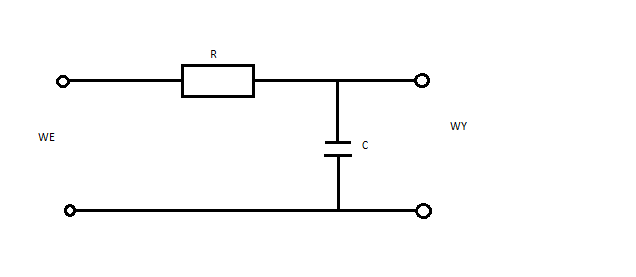
\includegraphics[width = 0.8\textwidth]{uklad.png}
		\caption{Schematyczny rysunek przedstawiający układ realizujący filtr dolnoprzepustowy.}
	\end{center}
\end{figure}

Do opisu tego układu wprowadza się pojęcie transmitancji. Jest ona zdefiniowana następująco:
$$ \alpha = |\frac{U_{out}}{U_{in}}| $$
W ogólności, ułamek pod modułem będzie liczbą zespoloną. Wtedy jego moduł odpowiada transmitancji, a argument (faza) przesunięciu fazowemu prądu wyjściowego. Dla naszego układu transmitancja będzie dana wzorem:
\begin{equation}
\alpha = \frac{1}{\sqrt{\omega^2R^2C^2 + 1} } ,
\end{equation} 
zaś przesuniecie fazowe:
\begin{equation}
 \phi = arctg(-\omega RC). 
\end{equation}
Dla filtru dolnoprzepustowego występuje pewna graniczną częstość $\omega_k$, dla której transmitancja przyjmuje wartość $\alpha = \frac{1}{\sqrt{2}} $

Aby wyznaczyć wartość krytyczną częstości musimy odwrócić wzór (1), tzn wyznaczyć $\omega (\alpha)$. Zależność tak wygląda następująco:
$$ \omega (\alpha) = \frac{\sqrt{1-\alpha^2}}{\alpha RC}, $$ a następnie 
wstawiając $\alpha = \frac{1}{\sqrt{2}}$ otrzymujemy:
\begin{equation} \omega_k = \frac{1}{RC} \end{equation}


Nazwa filtr dolnoprzepustowy wynika właśnie z tego, iż prądy o częstościach "dolnych" - tj. mniejszych od częstości granicznej są dobrze przepuszczane, zaś te o częstościach wyższych są silnie tłumione.
Z rozwiązania równań Kirkchoffa wynika również, iż napięcie wyjściowe 
dane będzie następującym wzorem:
$$U_{out}(t) = \frac{1}{RC} \int(U_{in}(t) - U_{out}(t)) dt, $$
a zatem dla $U_{out} \ll 1$ otrzymujemy
$$U_{out}(t) \approx \frac{1}{RC} \int U_{in}(t) dt. $$
Aby powyższe przybliżenie można było stosować, częstość musi być znacznie większa niż częstość graniczna, co zapewni nam, że $\frac{U_{out}}{U_{in}} \ll 1. $

\section*{Przebieg doświadczenia}
Obwód elektryczny, potrzebny do zbadania charakterystyki filtra został przygotowany na makiecie pomiarowej. Cały układ przedstawia schematyczny  Rys. 2.

\begin{figure}[ht!]	
	\begin{center}
		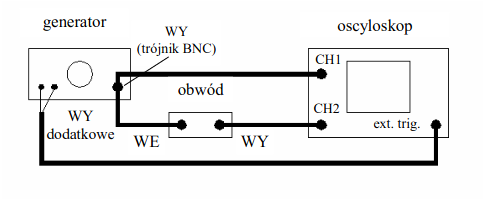
\includegraphics[width = 0.6\textwidth]{obwod.png}
		\caption{Schematyczny rysunek przedstawiający cały obwód służący do badania charakterystyk filtra dolnorzepustowego.}
	\end{center}
\end{figure}	

Na schemacie przez "obwód" został oznaczony element służący jako filtr.
W doświadczeniu zostały wykorzystane następujące urządzenia pomiarowe:
\begin{itemize}
\item generator funkcji prądu zmiennego
\item oscyloskop wielokanałowy
\item płytka montażona, umożliwiająca lutowanie elementów
\item opornik
\item kondensator
\item lutownica
\item miernik uniwersalny marki Brymen
\item przewody umożliwiające połączenie urządzeń
\end{itemize}
Przed doświadczeniem zostały zmierzone wartości oporu opornika oraz pojemności kondensatora. Wynoszą one:
$$ R_{zm} = 1.006 \pm 0.012 \ k\Omega \qquad C_{zm} = 95.30 \pm 3.94 \ nF. $$
Po podłączeniu wszystkich urządzeń i elementów zgodnie ze schematem, zebrano pomiary napięcia wejściowego oraz wyjściowego, a także przesunięcia fazowego tychże napięć. W tym doświadczeniu użyto metody "graficznej", tzn. wartości amplitud były odczytywane dla minimów/maksimów prądu, na podziałce oscyloskopu. Taka metoda jest niestety obarczona dużym błędem, co omówiono szerzej w następnych sekcjach.
Zakres częstotliwości, dla których wykonano pomiaru to 10kHz do 200kHz. Po zebraniu niezbędnych punktów pomiarowych dokonano porównania kształtu napięć, dla częstotliwości znacznie mniejszej niż częstotliwość graniczna (tu $f$=500Hz), oraz znacznie większej (tu $f$=200kHz). Na podstawie kształtu napięć potwierdzono tezę, iż dla wysokich częstotliwości filtr na wyjściu zwraca zcałkowany kształt prądu wejściowego. 
Tabela pomiarów została zawarta w dodatku A. Aby z pomiarów ($\delta$t) uzyskać przesunięcie fazowe, należy zastosować następujący wzór:
$$\phi = \frac{-2\pi dt}{T} = -2\pi dt f $$
\section*{Analiza danych}
Przy każdym pomiarze dla ustalonej częstotliwości $f$ zostały spisane trzy wartości liczbowe: napięcie wejściowe dostarczane przez generator funkcji ($U_{in}$), napięcie wyjściowe, czyli, tak jak według schematu na Rys. 1, spadek napięcia na kondensatorze ($U_{out}$), oraz przesunięcie fazowe pomiędzy tymi dwoma napięciami ($\phi$). We wszystkich przypadkach błąd pomiarowy został przyjęty jako najmniejsza podziałka skali na oscyloskopie, przy której została odczytana wartość pomiaru. Wartość częstotliwości uznajemy za dokładną. O ile przy pomiarach wartości natężenia nie było problemu z określeniem błędu, tak przy przesunięciu fazowym, szczególnie przy niskich częstotliwościach było to problematyczne, ponieważ wartości pomiarów dla kilku pierwszych serii wynoszą 0. Aby poradzić sobie z problemem niepewności w analizie danych zostały przyjęte arbitralne wartości błędu pomiarowego, które odpowiadają możliwym wartościom najmniejszych podziałek podczas zbierania pomiarów. \\
Pierwszym krokiem analizy danych było naniesienie danych pomiarowych na wykres oraz znalezienie parametrów dopasowania. Dla pomiarów napięcia została najpierw policzona wartość transmitancji dla każdego pomiaru. Wartość ta, przewidywana przez model teoretyczny jest opisana równaniem 	(1). Dla takiej funkcji dokonano dopasowania punktów pomiarowycj, co w rezultacie dało wartość parametru $RC$.
Poniższy wykres przedstawia dopasowaną zależność oraz punkty pomiarowe.

\begin{figure}[ht!]	
	\begin{center}
		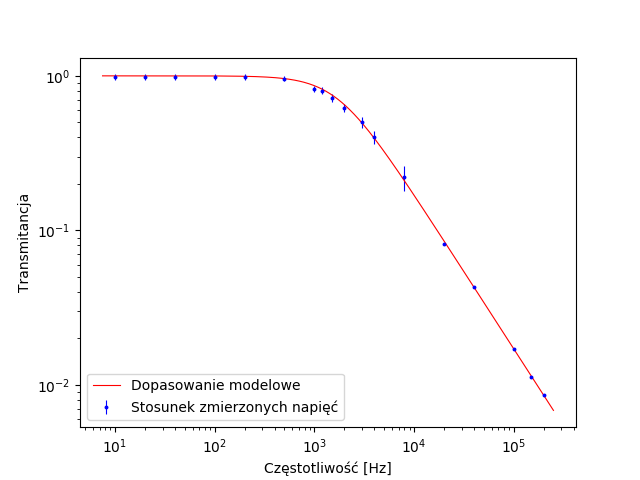
\includegraphics[width = 0.6\textwidth]{alpha.png}
		\caption{Wykres przedstawiający wyznaczone na podstawie pomiarów wartości transmitancji w zależności od częstotliwości sygnału wejściowego, oraz dopasowaną zależność teoretyczną.}
	\end{center}
\end{figure}	

Jak widać na Rys. 3, wyznaczony współczynnik $RC$ dobrze dopasowuje zależność teoretyczną do pomiarów. Korzystając z charakterystyki napięciowej współczynnik został wyznaczony jako:
$$ RC_{\alpha} = 92.93 \pm 0.19 \ \mu \text{s} $$
Możemy go porównać do rzeczywistego współczynnika, który policzyć można ze zmierzonych wartości oporu oraz pojemności:
$$ RC_{zm} = 95.9 \pm 4.1 \ \mu \text{s}, $$
Możemy dokonując test 3 sigma potwierdzić zgodność.
Porównując otrzymane wielkości oraz ich niepewności, możemy uznać, że dopasowany współczynnik dosyć dobrze pasuje do tego wynikającego ze zmierzonych wartości oporu oraz pojemności, a rozbierzność zostanie przedyskutowana poniżej. \\
Tę samą procedurę możemy powtórzyć, dla pomiarów przesunięcia fazowego. Teoretyczną zależność wynikającą z modelu opisuje wzór (2). Poniżej znajduje się rysunek (Rys.4) przedstawiający naniesione punkty pomiarowe oraz krzywą wynikającą z modelu teoretycznego, z dopasowanym współczynnikiem $RC$.

\begin{figure}[ht!]	
	\begin{center}
		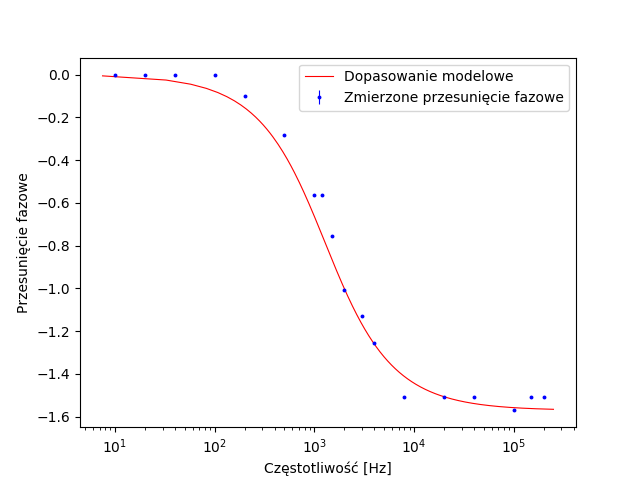
\includegraphics[width = 0.6\textwidth]{phi.png}
		\caption{Wykres przedstawiający obliczone na podstawie pomiarów wartości przesunięcia fazowego, zależnego od częstotliwości, oraz dopasowaną zależność teoretyczną.}
	\end{center}
\end{figure}	

Krzywa wynikająca z modelu teoretycznego i dopasanego doń parametru $RC_{\phi}$ znacznie bardziej odbiega od punktów pomiarowych, niż w przypadku transmitancji.
Obliczony współczynnik wynosi:
$$ RC_{\phi} = 124 \pm 21 \mu \text{s}. $$
Porównując go znowu do wartości wynikającej ze zmnierzonych wartości $R$ oraz $C$, możemy określić jak dobrze mu odpowiada. Tym razem współczynnik $RC$ jest dosyć mocno oddalony od faktycznego współczynnika. Można to wytłumaczyć słabą jakością pomiarów przesunięcia fazowego, wynikającą ze stosowanej metody, oraz faktu, iż przy bardzo niskich częstotliwościach wręcz niemożliwe było zauważenie przesunięcia fazowego, mimo że takowe mogło wystąpić. Warto wspomnieć też, że miejscami ciężko było zlokalizować gdzie dokładnie znajduje się minimum albo maksimum prądu, co mogło wpłynąć na pomiary. \\
Podsumowując, współczynnik $RC$ dopasowania modelowego możemy uznać za wiarygodny jedynie w przypadku pomiarów napięć / transmitancji. Pomiary przesunięcia fazowego faktycznie odtwarzają przewidywany kształt zależności, jednak liczbowo, z uwagi na błędy pomiarowe, nie możemy się na nich opierać.
Zatem za najlepsze wyznaczenie paramteru $RC$ dopasowania do modelu teoretycznego przyjmujemy wartość $RC_{\alpha} = 92.93 \pm 0.19 \ \mu \text{s} $. 
Błędy pomiarowe przesunięcia fazowego, zostały (jak już wyżej omówiono), wybrane arbitralnie na przedziale gdzie nie dało się odczytać przesunięcia, a w pozostałym zakresie przyjęto jako najmniejszą podziałkę częstotliwości na oscyloskopie. Konsekwencją jest niedoszacowanie błędu pomiarowegu przy tej metodzie, co objawia się np. na Rys.4, na którym prawie nie widać zaznaczonych błędów.
Podczas liczenia niepewności transmitancji zaś, zastosowano metodę propagacji małych błędów, która uwzględnia zależność funkcyjną transmitancji od mierzonych wielkości, oraz błędy tychże wielkości. Ma ona następującą postać:
$$ s_{\alpha i} = \sqrt{ (\frac{s_{out_i}}{U_{in_i}})^2 + (\frac{s_{in_i}}{U_{in_i}}\alpha_i)^2 } ,$$
gdzie $s_{\alpha i}$ to niepewność i-tej wartości transmitancji $\alpha$, $s_{out_i}$ to niepewność i-tego pomiaru napięcia wejściowego, 
$s_{in_i}$ to niepewność i-tego pomiaru napięcia wejściowego (ta niepewność była taka sama dla wszystkich pomiarów, ponieważ napięcie wejściowe się nie zmieniało), $U_{in_i}$ to i-ty pomiar napięcia wejściowego, zaś $\alpha_i$ to i-ta obliczona wartość transmitancji. \\
W celu wyznaczenia częstotliwości krytycznej odwołamy się do wzoru (3). 
$$ f_k = \frac{1}{2\pi RC}, $$
skąd po podstawieniu $RC_{\alpha}$ otrzymujemy:
$$ f_k = 1712.6 \pm 5.6 \ \text{Hz}. $$
Odpowiada to dosyć dobrze częstotliwości, dla której transmitancja zaczyna znacząco maleć. Widać to na wykresie z Rys.3.
Niepewność częstotliwości krytycznej została policzona korzystając z metody propagacji małych błędów, skąd wynika wzór:
$$ s_f = \frac{s_{RC}}{(2\pi RC)^2}$$

Można porównać otrzymaną częstotliwość graniczną dla wyznaczonej na podstawie zmierzonych wartości oporu oraz pojemności. 
$$ f_{zm} = 1660 \pm 11 \ \text{Hz} $$.

Warto nadmienić, iż dopasowania zależności wyznaczonych teoretycznie zostały przeprowadzone w języku Python (wersja 3.7), przy użyciu funkcji curve\_fit z pakietu scipy.optimize. Zastosowano metodę najmniejszych kwadratów, jako fukncję minimalizującą. \\

Po przeprowadzeniu wszystkich pomiarów zostało również sprawdzone, czy filtr działa "całkująco" dla częstotliwości większych niż krytyczna. W tym celu porównano kształt funkcji wejściowej oraz wyjściowej dla częstości $f$ = 200 kHz, który schematycznie pokazuje Rys. 5, oraz dla $f$ = 500 Hz, gdzie w tym przypadku nie można było zauważyć żadnej zależności różniczkująco - całkującej. 

\begin{figure}[ht!]	
	\begin{center}
		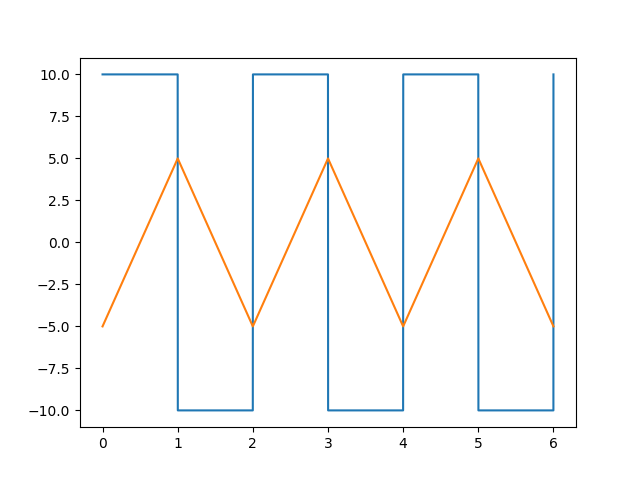
\includegraphics[width = 0.6\textwidth]{calka.png}
		\caption{Schematyczny wykres przedstawiający uzyskany kształt funkcji wyjściowej (kolor pomarańczowy) dla $f$ = 200kHz, oraz funkcji wejściowej (kolor niebieski). Skala niezachowana.}
	\end{center}
\end{figure}	

Potwierdziło to zatem hipotezę głoszącą, iż dla częstotliwości znacznie większych od częstotliwości granicznej, filtr zadziała jako układ całkujący kształt funkcji.

\section*{Podsumowanie}
Celem doświadczenia było sprawdzenie charakterystyki napięciowej filtru dolnoprzepustowego, zadanie to zostało pomyślnie wykonane. Na podstawie pomiarów udało się potwierdzić, iż badany układ posiada cechy filtra dolnoprzepustowego, tj. nie tłumi wartości poniżej krytycznej częstotliwości.
Ponadto udało się zmierzyć współczynnik $RC$, wykorzystany przy teoretycznym dopasowaniu modelu, wynosi on 
$$ RC_{\alpha} = 92.93 \pm 0.19 \ \mu \text{s}.$$
Charakterystyka fazowa również potwierdziła zależność modelową, lecz nie udało się z zadowalającą dokładnością wyciągąć ilościowych wniosków z jej analizy. Wynika to z metody wykorzystanej do zbierania pomiarów. W tym miejscu warto zaznaczyć, iż o wiele lepsze rezultaty udałoby się osiągnąć wykorzystując wbudowane funkcje oscyloskopu, m. in. odczytywanie odległośći pomiędzy wskazanymi punktami (wskaźniki). 
Na podstawie charakterystyki napięciowej udało się również wyznaczyć graniczną częstotliwość przenoszenia, wynosi ona:
$$ f_k = 1712.63 \pm 5.57 \ \text{Hz}. $$ Odbiega ona nieznacznie
od częstości wyznaczonej na podstawie zmierzonych wielkości $R$ oraz $C$, może to być spowodowane nieuwględnieniem impedancji generatora funkcji w rachunkach. częstotliwość krytyczna dla zmierzonych wielkości wynosi: $$ f_{zm} = 1660 \pm 11 \ \text{Hz}. $$


Na koniec doświadczenia
udało się potwierdzić hipotezę głoszącą, iż dla częstotliwości znacznie większych od granicznej, układ będzie "całkował" sygnał, który dostanie na wejściu. Zostało to zrobione w sposób jakościowy, porównując kształt prądu wejściowego i wyjściowego dla dużej częstości.


\section*{Dodatek A}

\begin{table}[htp!]
\begin{center}
\begin{tabular}{|c|c|c|c|c|c|}
\hline
	$f$ [Hz] & $U_{in}$ [V] & $U_{out}$ [V] & $s_{out}$ [V] & $\delta t$ [$\mu$s] & $ s_{\delta t}$ [$\mu$s] \\ \hline
	10.0 & 5.1 & 5.0 & 0.2 & 0.0 & 1000.0 \\ \hline
	20.0 & 5.1 & 5.0 & 0.2 & 0.0 & 750.0 \\ \hline
	40.0 & 5.1 & 5.0 & 0.2 & 0.0 & 500.0 \\ \hline
	100.0 & 5.1 & 5.0 & 0.2 & 0.0 & 250.0 \\ \hline
	200.0 & 5.1 & 5.0 & 0.2 & 80.0 & 40.0 \\ \hline
	500.0 & 5.1 & 4.9 & 0.2 & 90.0 & 20.0 \\ \hline
	1000.0 & 5.1 & 4.2 & 0.2 & 90.0 & 20.0 \\ \hline
	1200.0 & 5.0 & 4.0 & 0.2 & 75.0 & 10.0 \\ \hline
	1500.0 & 5.0 & 3.6 & 0.2 & 80.0 & 40.0 \\ \hline
	2000.0 & 5.0 & 3.1 & 0.2 & 80.0 & 40.0 \\ \hline
	3000.0 & 5.0 & 2.5 & 0.2 & 60.0 & 20.0 \\ \hline
	4000.0 & 5.0 & 2.0 & 0.2 & 50.0 & 20.0 \\ \hline
	8000.0 & 5.0 & 1.1 & 0.2 & 30.0 & 10.0 \\ \hline
	20000.0 & 5.0 & 0.41 & 0.02 & 12.0 & 4.0 \\ \hline
	40000.0 & 4.9 & 0.21 & 0.01 & 6.0 & 2.0 \\ \hline
	100000.0 & 4.9 & 0.084 & 0.004 & 2.5 & 1.0 \\ \hline
	150000.0 & 4.85 & 0.055 & 0.002 & 1.6 & 0.4 \\ \hline
	200000.0 & 4.85 & 0.042 & 0.002 & 1.2 & 0.2 \\ \hline
\end{tabular} 
\caption{Tabela zmierzonych wartości.} 
\end{center}
\end{table}



\end{document}